\cleardoublepage
\chapter{Evaluation} \label{chap:evaluation}
In order to evaluate the introduced mathematical meta-model and assess the impact of the Digital Shadow on ROS2 platforms, this chapter addresses various aspects, ranging from the feasibility of generating system specific models to utilisation tests under varying conditions. To this end, a proof-of-concept, which is based on the logical model presented in \Cref{sec:dshadow:logicalmodel}, is implemented\footnote{The implementation can be found at: \url{https://github.com/KARTOFF8xE/STREAM-DSM}.}.

\Cref{sec:evaluation:tools} briefly describes the frameworks and tools that are employed to implement the introduced approach. To align the evaluation with the objectives defined in \Cref{chap:motivation}, \Cref{sec:evaluation:mathmetamodel,sec:evaluation:challenges,sec:evaluation:limitations} address the objectives referring to the introduced meta-model. To elaborate, the meta-model aims to be applicable to a wide range of ROS2 systems, while enabling the integration of system specific information and creating holistic perspectives on the ROS2 system. Additionally, it is intended to accurately represent the dynamic nature of the running system. \Cref{sec:evaluation:mathmetamodel} illustrates the exemplary generation of a ROS2 system specific Shadow Instance. \Cref{sec:evaluation:challenges} describes challenges of the mathematical meta-model that predominantly originate from the employed tools, before constraints are derived from these challenges in \Cref{sec:evaluation:limitations}.\newline
The subsequent \Cref{sec:eval:performanceTests,sec:eval:requesting} address the objectives referring to the introduced Digital Shadow, which aims at minimising expert knowledge and the incurred performance overhead while being non-intrusive in order to keep the software stack and codebase clean. Therefore, \Cref{sec:eval:performanceTests} explores the performance of the Digital Shadow with respect to the generation of ROS2 system models. The overhead incurred due to processing requests, which gather information about the generated ROS2 system model, is explored in \Cref{sec:eval:requesting}.\newline
To further validate the applicability to real-world scenarios, \Cref{fig:eval:realWorld} explores the generation of a ROS2 system model within a real-world robot scenario.


In order to emphasise the feasibility of the mathematical meta-model, this chapter aligns with the legend defined in \Cref{chap:concept}. However, Members are now illustrated as visualised in \Cref{fig:neo4j:legend}. Note that Members of the ROS2 communication Graph are underlined. All figures that adhere to the updated legend are labelled with \circledLegend. Analogous to \legendadapted, \circledLegendadapted marks figures that adhere, but deviate from the legend in order to highlight specific characteristics.
\begin{figure}[h]
    \centering
    \hypertarget{target:circledLegend}{}
    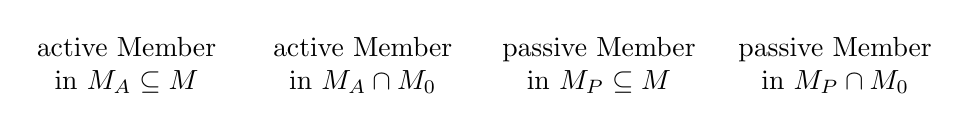
\begin{tikzpicture}
    \activeMember{foo}{(0,0)}{\phantom{/}…\phantom{/}}
    \node [align=center] at (0,-1.8) {active Member\\in $M_A \subseteq M$};
    \activeMember{foo}{(3,0)}{\phantom{/}\ul{…}\phantom{/}} % causal
    \node [align=center] at (3,-1.8) {active Member\\in $M_A \cap M_0$};
    \passiveMember{foo}{(6,0)}{\phantom{/}…\phantom{/}}
    \node [align=center] at (6,-1.8) {passive Member\\in $M_P \subseteq M$};
    \passiveMember{foo}{(9,0)}{\phantom{/}\ul{…}\phantom{/}} % causal
    \node [align=center] at (9,-1.8) {passive Member\\in $M_P \cap M_0$};
\end{tikzpicture}
    \caption[Partially Updated Legend]{Partially Updated Legend \circledLegend} \label{fig:neo4j:legend}
\end{figure}

\section{Employed Tools and Implementation} \label{sec:evaluation:tools}
    This section gives a brief overview of the tools employed in the proof-of-concept. Due to the focus of this thesis, it is implemented for ROS2.

    \begin{description}
        \item[ROS2 Version] \hfill \\
            In order to generate a ROS2 system specific model that represents the communication structure of the system, the tracepoints within the ROS2 source code are employed. As new tracepoints are exclusively added to the development version of ROS2 --~rolling~--, this version is utilised for the proof-of-concept. Nevertheless, it is important to mention that the implementation works independently of the ROS2 version, as long as the employed tracepoints exist. The utilised tracepoints are briefly described in  \Cref{tab:tracepoints}.\newline
        \item[The Shadow Caster] \hfill \\
            To generate an accurate Shadow Instance and prove the functionality of the logical model introduced in \Cref{subsec:dshadow:logical:caster}, the Digital Shadow strictly adheres to this logical model. The \fboxemph{Tracer} module of the Shadow Caster is represented by a \emph{structural tracer} and a \emph{continuous tracer}, tracing structural and continuous data of the ROS2 system in question, respectively. This distinction enhances the strict separation of structure and value, which thereby continues consistently throughout the approach of this thesis.\newline
            The structural and continuous tracer employ the Unix-exclusive \emph{LTTng} (Linux Trace Toolkit next generation) framework \cite{website:lttng} as the default tracing backend due to its low overhead capabilities in addition to its functionality for tracing both userspace and kernel events \cite{website:lttng}\cite{lttng}. Additionally, LTTng supports enabling and disabling tracepoints at runtime, thereby contributing to the objective of aggregating only necessitated data.\newline
            \emph{Babeltrace2} \cite{website:babeltrace} is selected as the parsing toolkit for recorded tracepoint events, as it is the toolkit recommended by LTTng for parsing recorded trace data \cite{website:lttng}. Tracepoint events are events that are triggered when an enabled tracepoint is reached and thus traced.\newline
            The proof-of-concept only contains the basic functionality that is necessitated to evaluate the concepts introduced in this thesis, with focus on the generation of platform-specific system models. For instance, the configurations that enable the integration of expert knowledge in the form of textual Requirement-Diagrams are not implemented. Inherently, the \fboxemph{Evaluator} module is not implemented.
        \item[The Shadow Instance] \hfill \\
            To represent the Shadow Instance, the graph database \emph{neo4j} \cite{website:neo4j} is employed to store the structural information of the model, as it is considered one of the most widely used graph databases in the world \cite[p.~377]{neo4jWidelyUsed}, which underlines its relevance and suitability for modelling structural information in practical applications.\newline
            Continuous numerical values are stored within the time-series database \emph{influxDB} \cite{website:influxdb}, which is chosen due to its low space consumption and high throughput capabilities \cite[p.~13]{influxdbPerformance}, thereby contributing to the objective of generating a lightweight solution.\newline
            The log database, for storing textual values, is not implemented. However, it is not necessitated to explore the viability of the proposed mathematical meta-model and the logical model of the Digital Shadow targeting ROS2 systems. This is because it fulfills an analogous function to the numerical time-series database with the exception that it additionally aims at the capability of storing exchanged ROS2 messages.\newline
        \end{description}

        In the present section, the combination of Shadow Caster and Shadow Instance is denoted as the \emph{Shadow Implementation}.

        Within the Shadow Implementation, the continuous values \glqq{}publishing rate\grqq{} and \glqq{}CPU utilisation\grqq{} are implemented to represent one ROS2 specific attribute and one operating system specific attribute. Thus one Edge-related attribute and one Member-related attribute are represented. The \glqq{}publishing rate\grqq{} is determined by the respective tracepoint, whereby the respective triggered events are analysed and assigned to a respective Publisher and thus publishing Edge. Therefore, the number of respective occurrences per second is computed to a respective publishing rate. The CPU utilisation is calculated by employing the information provided within the \emph{/proc} directory.\newline
        Additionally, the namespace- and process-driven, edge-induced Trees are implemented in order to evaluate their feasibility.

Based on the tools and frameworks employed, the subsequent sections explore the capabilities of the implementation in relation to the concepts proposed in this thesis. First and foremost, the following section focuses on evaluating the feasibility of the mathematical meta-model.


\section{Feasibility of the Mathematical Meta-Model} \label{sec:evaluation:mathmetamodel}
    The feasibility of the mathematical meta-model is imperative for achieving the objectives of this thesis. Therefore, this section gradually explores its feasibility by generating an exemplary ROS2 Graph in \Cref{subsec:eval:actionExample}. Subsequently, the implementation of aggregating the ROS2 system is described (\Cref{subsec:eval:aggregation}) before delving into the representation of continuous values in \Cref{sec:eval:continuousValues}. The potential for integrating system specific information is discussed in \Cref{subsec:eval:integratingInformation}.
    
    \vspace{-.125cm}
    \subsection{Generating an Exemplary ROS2 Graph} \label{subsec:eval:actionExample}
    \vspace{-.125cm}
    To demonstrate an application of the mathematical meta-model, an exemplary ROS2 Graph is generated for the official Action Server/Client tutorial \cite{website:acttutorial} of ROS2, as it offers a clear yet comprehensive insight into the communication within a ROS2 system. To this end, it is described gradually within this section. To ensure a clear understanding, the order stated does not correspond to the order in which the initialisation actually takes place.

    \begin{description}[leftmargin=\descriptionIndent, itemsep=-0.2em]
        \item [1) Instantiating Nodes] \hfill \\
        As a first step, two active Members, referring to the two initialised Nodes, are instantiated by the respective tracepoint events, which contain the Nodes respective namespace, name and handle. The process ID is gathered through contextual information. \Cref{fig:neo4j:exemplarygraph:nodes} illustrates the so far generated ROS2 Graph. Note that the instantiated active Members are not part of the ROS2 communication Graph, as they are not connected to any communication Edges.
        \begin{figure}[h]
            \centering
            \begin{tikzpicture}
    \activeMember{actSrv}{( 2,0)}{fib\_act\_srv}
    \activeMember{actCli}{(-2,0)}{fib\_act\_cli}
\end{tikzpicture}
            \caption[Instantiating Active Members that Represent Nodes]{Instantiating Active Members that Represent Nodes \circledLegend} \label{fig:neo4j:exemplarygraph:nodes}
        \end{figure}
        \item [2) Instantiating Timers] \hfill \\
        Timers are created by two tracepoint events, whereby one instantiates the Timer and thereby establishes a correlation between the Timer's handle and frequency. Concurrently, the second event establishes a link between the respective Node handle and Timer handle. Note that the Action Client is connected to at least one communication Edge and therefore part of the ROS2 communication Graph (\Cref{fig:neo4j:exemplarygraph:action}).
        \begin{figure}[h]
            \centering
            \begin{tikzpicture}
    \activeMember{actSrv}{( 2,0)}{fib\_act\_srv}
    \activeCausalMember{actCli}{(-2,0)}{fib\_act\_cli}
    \CommunicationTimer{actCli}{160}
    \CommunicationTimer{actCli}{200}
\end{tikzpicture}
            \caption[Adding Timers to the Generated ROS2 Graph]{Adding Timers to the Generated ROS2 Graph \circledLegend} \label{fig:neo4j:exemplarygraph:timer}
        \end{figure}
        \enlargethispage{1\baselineskip}
        \item [3) Instantiating Services] \hfill \\
        To represent Services, six sending Edges are added between the active Members, referring to the request and response of the individual Services \glqq{}send\_goal\grqq{}, \glqq{}cancel\_goal\grqq{}, and \glqq{}get\_result\grqq{}. The Service Server/Client communication is instantiated by two tracepoint events.\clearpage Both contain the name of the associated Service Server in addition to the respective Node handle. The tracepoints are differentiated by their purpose, whereby one induces the instantiation of a Service Client and thus additionally provides a respective Client handle, while the second induces the instantiation of a Service Server and thus provides a respective Server handle. \Cref{fig:neo4j:exemplarygraph:service} illustrates the updated ROS2 Graph containing the newly added sending Edges. Note that even though there are multiple sending Edges in both directions, each Edge is individually identified by the name of the Service Server/Client combination it relates to. This aspect is important for later analyses.
        \begin{figure}[h]
            \centering
            \begin{tikzpicture}

    \activeCausalMember{actcli}{(-4,0)}{action-cli}
    \activeCausalMember{actsrv}{(4,0)}{action-srv}
    \CommunicationTimer{actcli}{160}
    \CommunicationTimer{actcli}{200}

    \curvedEdgeWithProperties{actcli}{actsrv}{\textit{send\_goal} (req)}{33}{G0, thick}
    \curvedEdgeWithProperties{actsrv}{actcli}{\textit{send\_goal} (resp)}{-20}{G0, thick}
    \curvedEdgeWithProperties{actcli}{actsrv}{\textit{get\_result} (req)}{7}{G0, thick}
    \curvedEdgeWithProperties{actsrv}{actcli}{\textit{get\_result} (resp)}{7}{G0, thick}
    \curvedEdgeWithProperties{actcli}{actsrv}{\textit{cancel\_goal} (req)}{-20}{G0, thick}
    \curvedEdgeWithProperties{actsrv}{actcli}{\textit{cancel\_goal} (resp)}{33}{G0, thick} 

\end{tikzpicture}
            \caption[Adding Sending Edges that Represent Server-Client Communication]{Adding Sending Edges that Represent Server-Client Communication \circledLegend} \label{fig:neo4j:exemplarygraph:service}
        \end{figure}
        \item [4) Instantiating Topics] \hfill \\
        A variety of Topics, relating to passive Members, is added to the existing Graph. However, Topics are not created explicitly, they are initialised alongside the instantiation of a Publisher or Subscriber. The respective tracepoint events contain the handle of the initialising Node, the handle of the respective Publisher or Subscriber, and the name of the respective Topic. The updated ROS2 Graph is illustrated within \Cref{fig:neo4j:exemplarygraph:action}. Note that only the upper two Topics refer to the concept of Actions. The lower two Topics are fundamental Topics any ROS2 Node publishes and subscribes to.
        \begin{figure}[h]
            \centering
            \begin{tikzpicture}
    \activeCausalMember{actCli}{(-4,0)}{action-cli}
    \activeCausalMember{actSrv}{( 4,0)}{action-srv}
    \CommunicationTimer{actCli}{160}
    \CommunicationTimer{actCli}{200}

    \passiveCausalMember{feedback}{(-2.5, 2.75)}{feedback}
    \passiveCausalMember{status}  {( 2.5, 2.75)}{status}
    \passiveCausalMember{rosout}  {( 2.5,-2.75)}{rosout}
    \passiveCausalMember{paramEv} {(-2.5,-2.75)}{paramEv}

    \curvedEdgeWithProperties{actCli}{actSrv}{\textit{send\_goal} (req)}{33}{G0, thick}
    \curvedEdgeWithProperties{actSrv}{actCli}{\textit{send\_goal} (resp)}{-20}{G0, thick}
    \curvedEdgeWithProperties{actCli}{actSrv}{\textit{get\_result} (req)}{7}{G0, thick}
    \curvedEdgeWithProperties{actSrv}{actCli}{\textit{get\_result} (resp)}{7}{G0, thick}
    \curvedEdgeWithProperties{actCli}{actSrv}{\textit{cancel\_goal} (req)}{-20}{G0, thick}
    \curvedEdgeWithProperties{actSrv}{actCli}{\textit{cancel\_goal} (resp)}{33}{G0, thick}

    \curvedEdgeWithProperties{actSrv}  {status}{}{-15}{G0, thick}
    \curvedEdgeWithProperties{actSrv}  {feedback}{}{-20}{G0, thick}
    \curvedEdgeWithProperties{status}  {actCli}{}{-20}{G0, thick}
    \curvedEdgeWithProperties{feedback}{actCli}{}{-15}{G0, thick}

    \curvedEdgeWithProperties{actSrv}{rosout}{}{15}{G0, thick}
    \curvedEdgeWithProperties{actSrv}{paramEv}{}{15}{G0, thick}
    \curvedEdgeWithProperties{actCli}{rosout}{}{-15}{G0, thick}
    \curvedEdgeWithProperties{actCli}{paramEv}{}{-15}{G0, thick}

    \curvedEdgeWithProperties{rosout}{actSrv}{}{-35}{G0, thick}
    \curvedEdgeWithProperties{paramEv}{actSrv}{}{-24}{G0, thick}
    \curvedEdgeWithProperties{rosout}{actCli}{}{24}{G0, thick}
    \curvedEdgeWithProperties{paramEv}{actCli}{}{35}{G0, thick}
\end{tikzpicture}
            \caption[Extending the Example by Topics Represented as Passive Members]{Extending the Example by Topics Represented as Passive Members \circledLegend} \label{fig:neo4j:exemplarygraph:action}
        \end{figure} \enlargethispage{1\baselineskip}
        

        \hspace{-\descriptionIndent}\parbox{\textwidth}{The ROS2 communication Graph representing the communication structure of the official Action Server/Client tutorial is thus fully represented. However, as mentioned in \Cref{sec:evaluation:tools}, the process- and namespace-driven Trees are integrated into the Graph's structure to organise the ROS2 Graph (see \Cref{subsec:mathModel:trees}). For the sake of clarity, the communication Edges are not explicitly named in further figures.}

        \item[5) Integrating the Process-Driven Tree] \hfill \\
        The process-driven Tree is integrated into the existing ROS2 communication Graph by inserting additional Members and organising Edges that represent the various affiliated processes and their relationships. It is constructed by joining the roots of several Subtrees. Each Subtree consists of multiple branches, which are constructed by recursively traversing the parent processes of the respective process instance that encompasses a Node. It is trimmed above the least process called \glqq{}ros2\grqq{}. As a result, each branch starts with the respective process instance that encompasses a Node and ends at the least process called \glqq{}ros2\grqq{}. Subsequent to the traversal and trimming, the thus created branch of the Tree is added to the respective Subtree. Within \Cref{fig:neo4j:exemplarygraph:processdrivenTree}, the active Members called \glqq{}ros2\grqq{} relate to the instances that triggered the Action Server and Action Client, respectively\footnote{Both were started via a \emph{ros2 run} command.}. Note the passive Member called \glqq{}host\grqq{}, which relates to the virtual and thus passive Member that joins all Subtrees that originate from the same operating system.
        \begin{figure}[h]
            \centering
            \input{figures/tikz/neo4j/processDrivenTree.tex}
            \caption[Extending the ROS2 Graph by its Respective Process-Driven Tree]{Extending the ROS2 Graph by its Respective Process-Driven Tree \circledLegend} \label{fig:neo4j:exemplarygraph:processdrivenTree}
        \end{figure}

        \item[6) Integrating the Namespace-Driven Tree] \hfill \\
        The namespace-driven Tree is constructed based on the name structure of each communication Member. For instance, the fully qualified name of the \glqq{}feedback\grqq{}-Topic relates to \glqq{}/action/fibonacci/feedback\grqq{}, which is split into its components \glqq{}/\grqq{}, \glqq{}action/\grqq{}, \glqq{}fibonacci/\grqq{}, and \glqq{}feedback\grqq{}. The first component refers to the root of the namespace-driven Tree, which is represented by a passive Member called \glqq{}/\grqq{}. The second component is represented by a passive Member called \glqq{}action\grqq{}, which is connected to the root via an organising Edge. The third component is represented by a passive Member called \glqq{}fibonacci\grqq{}, which is connected to the second component via an organising Edge. Finally, the fourth component, called \glqq{}feedback\grqq{}, represents the Topic as a passive Member and is connected to the third component via a further organising Edge. This process is repeated for all communication Members, thereby creating a Tree structure that represents the namespace structure of the ROS2 system. The exemplary, resulting namespace-driven Tree is added to the so far constructed Graph, visualised in \Cref{fig:neo4j:fullExemplaryGraph}.
        \begin{figure}[h]
            \centering
            \begin{tikzpicture}
    \passiveMember{processRoot}{(0,0)}{host}
    \activeMember{ros2a}{(2, 2)}{ros2}
    \activeMember{ros2b}{(2, -2)}{ros2}
    \activeCausalMember{actSrv}{(4.5,2)}{fib\_act\_srv}
    \activeCausalMember{actCli}{(4.5,-2)}{fib\_act\_cli}

    \passiveMember{namespaceRoot}{(12.5,-2)}{/}
    \passiveMember{action}{(12.5,2)}{action/}
    \passiveMember{fibonacci}{(10.2,2)}{fibonacci/}
    \passiveCausalMember{status}{(8,1)}{status}
    \passiveCausalMember{feedback}{(8,3)}{feedback}
    \passiveCausalMember{rosout}{(8,-1)}{rosout}
    \passiveCausalMember{paramEv}{(8,-3)}{paramEv}

    \curvedEdgeWithProperties{processRoot}{ros2a}{}{0}{TreeProcess}
    \curvedEdgeWithProperties{processRoot}{ros2b}{}{0}{TreeProcess}
    \curvedEdgeWithProperties{ros2a}{actSrv}{}{0}{TreeProcess}
    \curvedEdgeWithProperties{ros2b}{actCli}{}{0}{TreeProcess}

    \curvedEdgeWithProperties{namespaceRoot}{action}{}{0}{TreeNamespace}
    \curvedEdgeWithProperties{action}{fibonacci}{}{0}{TreeNamespace}
    \curvedEdgeWithProperties{fibonacci}{feedback}{}{0}{TreeNamespace}
    \curvedEdgeWithProperties{fibonacci}{status}{}{0}{TreeNamespace}
    \curvedEdgeWithProperties{namespaceRoot}{paramEv}{}{0}{TreeNamespace}
    \curvedEdgeWithProperties{namespaceRoot}{rosout}{}{0}{TreeNamespace}
    \curvedEdgeWithProperties{namespaceRoot}{actSrv}{}{0}{TreeNamespace}
    \curvedEdgeWithProperties{namespaceRoot}{actCli}{}{0}{TreeNamespace}

    \curvedEdgeWithProperties{actSrv}{actCli}{}{25}{G0, thick}
    \curvedEdgeWithProperties{actCli}{actSrv}{}{-15}{G0, thick}
    \curvedEdgeWithProperties{actSrv}{actCli}{}{5}{G0, thick}
    \curvedEdgeWithProperties{actCli}{actSrv}{}{5}{G0, thick}
    \curvedEdgeWithProperties{actSrv}{actCli}{}{-15}{G0, thick}
    \curvedEdgeWithProperties{actCli}{actSrv}{}{25}{G0, thick}

    \curvedEdgeWithProperties{actSrv}{feedback}{}{0}{G0, thick}
    \curvedEdgeWithProperties{actSrv}{status}{}{0}{G0, thick}
    \curvedEdgeWithProperties{feedback}{actCli}{}{0}{G0, thick}
    \curvedEdgeWithProperties{status}{actCli}{}{0}{G0, thick}
    
    \curvedEdgeWithProperties{actSrv}{rosout}{}{3}{G0, thick}
    \curvedEdgeWithProperties{actCli}{rosout}{}{3}{G0, thick}
    \curvedEdgeWithProperties{actSrv}{paramEv}{}{3}{G0, thick}
    \curvedEdgeWithProperties{actCli}{paramEv}{}{3}{G0, thick}

    \curvedEdgeWithProperties{rosout}{actSrv}{}{3}{G0, thick}
    \curvedEdgeWithProperties{rosout}{actCli}{}{3}{G0, thick}
    \curvedEdgeWithProperties{paramEv}{actSrv}{}{3}{G0, thick}
    \curvedEdgeWithProperties{paramEv}{actCli}{}{3}{G0, thick}

    \CommunicationTimerNoText{actCli}{-70}
    \CommunicationTimerNoText{actCli}{-120}
\end{tikzpicture}
            \caption[Extending the ROS2 Graph by its Respective Namespace-Driven Tree]{Extending the ROS2 Graph by its Respective Namespace-Driven Tree \circledLegend} \label{fig:neo4j:fullExemplaryGraph}
        \end{figure}
        
    \end{description}

    This section demonstrated the feasibility of the mathematical meta-model for representing the fundamentals of ROS2 systems. Specifically, it generated a system specific model that reflects the communication structure created in the Action Server/Client tutorial. Additionally, the respective process- and namespace-driven Trees have been integrated into the ROS2 Graph.\newline
    With the evidence that the implementation is capable of representing the fundamental structure of ROS2 systems, the subsequent section describes the implementation of the aggregations and summations (see \Cref{sec:mathModel:aggregation}).

\vspace{-.125cm}
    \subsection{Aggregating ROS2 Systems} \label{subsec:eval:aggregation}
\vspace{-.125cm}
        The aggregations defined in \Cref{sec:mathModel:aggregation} are intended to facilitate \acl{fdd} by enabling a broad but blurred view of the ROS2 system in question. Thus, their feasibility is imperative to the objectives of this thesis, as they enable a holistic view onto a ROS2 system.

        All aggregations are implemented by first querying the graph database in order to retrieve the respective Members and Edges. Subsequently, as each aggregation leads to a totalling of the respective attribute values, the time-series database is queried to directly total the respective attribute values and return the computed result.\newline
        An exemplary aggregation and its influence on the involved systems is represented in \Cref{subsec:eval:requestAggregation}.

        With the computations defined in the mathematical meta-model implemented, the following section explores the integration of time-dependent and thus continuous values.


    \subsection{Continuous Values in the ROS2 Digital Shadow} \label{sec:eval:continuousValues}
        As described previously, the strict separation of structure and continuous values is maintained throughout the entire approach of this thesis. Within the ROS2 Graph, each Member and communication Edge is provided with a UID, enabling an unambiguous assignment of attribute value to a respective entity. For instance, \Cref{fig:tikz:eval:continuousValues} illustrates the attribute values that refer to the publishing rates that are assigned to publishing Edges in order to illustrate the communication via Topics during an exemplary execution of the Action Server/Client tutorial (\Cref{fig:neo4j:fullExemplaryGraph}). The sequence of the Action Server returning its feedback to the Action Client is illustrated. Concurrently with the start of the feedback loop, the Action Server publishes the respective state of the Action procedure onto the \glqq{}status\grqq{}-Topic. In total, it publishes nine feedback messages to the respective \glqq{}feedback\grqq{}-Topic. Following the last message, the Action Server updates the state of the Action procedure by publishing onto the \glqq{}status\grqq{}-Topic again. Note also the six messages that the Action Client published onto the \glqq{}paramEv\grqq{}-Topic. Those messages were sent due to the initialisation of the Action Client.
        \begin{figure}[h]
            \centering
            \begin{tikzpicture}
\begin{axis}[
    name=second,
    xlabel={Relative Time [s]},
    ylabel={Publishing Rate [Hz]},
    tick align=center,
    legend style={
        at={(.5,1.05)},
        anchor=south,
        legend columns=3,
        font=\small,
        draw=black,
        font=\footnotesize
    },
    xtick distance=1,
    % minor ytick={0.5,1.5,...,5},
    % ytick distance=1,
    xmin=0, xmax=11,
    ymin=0, ymax=7,
    grid=both,
    height=4cm,
    width=14cm,
    xtick pos=bottom,
    ytick pos=left,
    ytick={0,1,6}
]

    \addplot+ [
        only marks,
        mark=*,mark options={solid},
        mark size=4.5,
        fill=tubaf-black,
        draw=tubaf-black,
        thick
    ] table [
        x=relTime,
        y=status,
        col sep=comma
    ] {measurements/publisherFrequency.csv};
    \addlegendentry{fib\_act\_src $\trianglearrow$ status}

    \addplot+ [
        only marks,
        mark=*,mark options={solid},
        mark size=2.5,
        fill=tubaf-environment,
        draw=tubaf-environment,
        thick,
    ] table [
        x=relTime,
        y=paramEvents,
        col sep=comma
    ] {measurements/publisherFrequency.csv};
    \addlegendentry{fib\_act\_cli $\trianglearrow$ paramEv}
    \addplot+ [
        only marks,
        mark=*,mark options={solid},
        mark size=2.5,
        draw=tubaf-material,
        fill=tubaf-material,
        thick
    ] table [
        x=relTime,
        y=feedback,
        col sep=comma
    ] {measurements/publisherFrequency.csv};
    \addlegendentry{fib\_act\_src $\trianglearrow$ feedback}

\end{axis}
\end{tikzpicture}
            \caption{Exemplary Publishing Rate of all Instances in the Generated ROS2 System Model} \label{fig:tikz:eval:continuousValues}
        \end{figure}\newline
        This strict separation of continuous values and structure, and the assignment via an UID, contributes to the objectives of this thesis, as it enables the selection of optimised solutions for both dimensions, i.e. storing structural values in a graph database and storing continuous, numerical values within a time-series database.


    With the evidence that the differentiation between structure and value is feasible, the subsequent section discusses the viability of integrating system specific information.


    \subsection{Integrating System Specific Information into the Model} \label{subsec:eval:integratingInformation}
        Due to its generic design, the mathematical meta-model can incorporate platform-specific elements into the generated ROS2 system model. This is achieved by treating externally integrated Members as equivalent to native ROS2 components. Therefore, externally integrated Members are also distinguished by the UID, which further enables a clear assignment to the continuous values stored within the time-series database, allowing for a seamless and coherent system representation.


    This section demonstrated the generation of an exemplary ROS2 Graph, gave a brief insight into the implementation of the aggregations and discussed the potential of integrating system specific information. Despite the promising results, the creation of a specific ROS2 system model is not without challenges. The subsequent section elaborates the challenges that arise when generating a system specific model based on the implemented proof-of-concept.


\section{Challenges while Generating System Specific Models} \label{sec:evaluation:challenges}
    The structure of the ROS2 communication Graph is exclusively generated by employing the tracepoints of the ROS2 source code.
    However, although the tracepoints appear to enable a faithful generation of the ROS2 Graph, there are challenges that may cause the model to degenerate.


    \subsection{Reassigning Communication Edges across Multiple Restarts}
        As described in \Cref{subsec:mathModel:versioning}, the ROS2 Graph is only populated and never reduced. Therefore, its Members and Edges are to be reassigned at the restart of the referring entity. For instance, if a Node terminates, its respective active Member and adjacent Edges are not removed and thus the topology of the ROS2 Graph is not changed. If the Node is restarted, it has to be reassigned to the respective active Member that it was represented by in the ROS2 Graph. Analogously, the instantiated Publishers, Subscribers, Service Servers, etc. are to be reassigned to their respective communication Edges. This is imperative, as information, like continuous values, is related to the specific entity throughout the entire runtime of the system.

        While this reassociation is trivial for communication Edges that are uniquely identified by their source, destination, type, and --~when existing~-- name\footnote{For instance, the name of a Service Server that is related to a sending Edge.}, this becomes challenging for communication Edges that cannot be separated by those properties.\newline
        To elaborate, consider a Node that manages five Publishers to the same Topic. Three of those Publishers are instantiated at the initialisation of the Node. The further Publishers are instantiated during runtime.\newline
        Reassigning the former three Publishers to their representations within the ROS2 Graph is trivial, as those Publishers are initialised within a given order and thus countable. This count is illustrated in \Cref{fig:tikz:pubProblem1}. However, there is no unambiguous property that differentiates the latter two Publishers, as there is no guarantee regarding their instantiation order (\Cref{fig:tikz:pubProblem2}). Thus, the reassignment of those Publishers to their respective publishing Edges presents a challenge.
        \begin{figure}[h]
            \centering
            \begin{subfigure}[h]{.48\textwidth}
                \centering
                \input{figures/tikz/neo4j/pubProblem/pubProblem1.tex}
                \caption[Exemplary, ROS2 Communication Graph Past Node Initialisation]{Exemplary, ROS2 Communication Graph Past Node Initialisation \circledLegend} \label{fig:tikz:pubProblem1}
            \end{subfigure}
            \begin{subfigure}[h]{.48\textwidth}
                \centering
                \begin{tikzpicture}
    \activeCausalMember{pub}{(0,0)}{talker}
    \passiveCausalMember{topic}{(5,0)}{topic}

    \curvedEdgeWithProperties{pub}{topic}{\textit{0}}{30}{G0, thick}
    \curvedEdgeWithProperties{pub}{topic}{\textit{1}}{15}{G0, thick}
    \curvedEdgeWithProperties{pub}{topic}{\textit{2}}{0}{G0, thick}
    \curvedEdgeWithProperties{pub}{topic}{\textit{?}}{-15}{G0, thick}
    \curvedEdgeWithProperties{pub}{topic}{\textit{?}}{-30}{G0, thick}
\end{tikzpicture}
                \caption[Exemplary, ROS2 Communication Graph During Runtime]{Exemplary, ROS2 Communication Graph During Runtime \circledLegend} \label{fig:tikz:pubProblem2}
            \end{subfigure}
            \caption[Challenge with Reassigning Communication Edges across Multiple Restarts]{Challenge with Reassigning Communication Edges across Multiple Restarts} \label{fig:tikz:pubProblem}
        \end{figure}


    \subsection{Differentiating between Multiple Message Types of a Single Topic}
        A second challenge arises from the ambiguity of Topic types (see \Cref{subsec:model:topics}). Since the tracepoint events that reflect the instantiation of Publishers or Subscribers for a given Topic do not provide any information about the respective message type they are transmitting or receiving, no differentiation between these types can be made.\newline
        For instance, consider a Topic that forwards messages of various types. As the generated ROS2 Graph contains no information about the message types, the resulting communication structure becomes degenerated. This is because a Node that subscribes to a Topic may not receive all messages published onto it. This challenge is illustrated in \Cref{fig:tikz:topicProblem}, where the publishing and subscribing Edges are coloured brown and green to represent different message types being published to the same Topic.
        \begin{figure}[h]
            \centering
            \begin{tikzpicture}
    \activeCausalMember{pub1}{(0,1)}{talker1}
    \activeCausalMember{pub2}{(0,-1)}{talker2}
    \passiveCausalMember{topic}{(4,0)}{topic}
    \activeCausalMember{sub1}{(8,1)}{listener1}
    \activeCausalMember{sub2}{(8,-1)}{listener2}

    \curvedEdgeWithProperties{pub1}{topic}{}{0}{tubaf-environment}
    \curvedEdgeWithProperties{pub2}{topic}{}{0}{tubaf-geo}
    \curvedEdgeWithProperties{topic}{sub1}{}{0}{tubaf-environment}
    \curvedEdgeWithProperties{topic}{sub2}{}{0}{tubaf-geo}
\end{tikzpicture}
            \caption[Challenge of Differentiating Multiple Message Types on a Single Topic]{Challenge of Differentiating Multiple Message Types on a Single Topic \circledLegendadapted} \label{fig:tikz:topicProblem}
        \end{figure}


    \subsection{Generating the Process-Driven, Edge-Induced Tree}
        The construction of the process-driven Tree induces a challenge that originates from the usage of Node Composition, where multiple Nodes are containerised and thus grouped within a single process to enhance system performance (see \Cref{sec:model:containers}). To elaborate, consider two Nodes as part of a Container and thus two Nodes that share the same process (\Cref{fig:tikz:processProblem}). If \glqq{}node1\grqq{} initiates the creation of a third Node (\glqq{}child\grqq{}), the parent process of \glqq{}child\grqq{} refers to both Nodes of the Container. In conclusion, \glqq{}child\grqq{} is assigned to two parent processes and the Tree is malformed.
        \begin{figure}[h]
            \centering
            \begin{tikzpicture}
    \activeMember{launch}{(-4,0)}{launch file}
    \activeCausalMember{pub1}{(0,1)}{node1}
    \activeCausalMember{pub2}{(0,-1)}{node2}
    \activeCausalMember{topic}{(4,0)}{child}

    \curvedEdgeWithProperties{launch}{pub1}{}{0}{TreeProcess}
    \curvedEdgeWithProperties{launch}{pub2}{}{0}{TreeProcess}
    
    \curvedEdgeWithProperties{pub1}{topic}{}{0}{TreeProcess}
    \curvedEdgeWithProperties{pub2}{topic}{}{0}{TreeProcess}

    \draw [rounded corners] (-1.2,-2) rectangle (1.2,2) node [above] at (0,2) {Container};

    \node [tubaf-energy] at (2.4,0) {\Huge !};
\end{tikzpicture}
            \caption[Challenge while Constructing the Process-Driven, Edge-Induced Tree]{Challenge while Constructing the Process-Driven, Edge-Induced Tree \circledLegendadapted} \label{fig:tikz:processProblem}
        \end{figure}


    \section{Defining Constraints on ROS2 Systems to Ensure Consistency and Correctness of the Generated Model} \label{sec:evaluation:limitations}
    In consideration of the constraints arising from the tools that are employed, it is imperative to define constraints for ROS2 systems in order to ensure the validity of the generated model. Therefore, the following constraints are defined.
        \begin{description}
            \item [The Combination of Name and Namespace of Nodes has to be Unique] \hfill \\
                Nodes are integrated into the model by employing the tracepoints of the ROS2 source code. The respective tracepoint events only provide the name and namespace of the Node to uniquely identify it across restarts. Therefore, the combination of the Node's name and namespace has to uniquely identify the Node.
            \item [Service Names have to be Unique] \hfill \\
                Similar to Nodes, Services are integrated into the model by employing the tracepoints of the ROS2 source code. The respective tracepoint events only provide the name of the Service to uniquely identify it across restarts. Thus, the Service is identified by its name only. In conclusion, the name of a Service has to be unique.
            \item [Topics are Required to have a Unique Type] \hfill \\
                Topics are implicitly instantiated alongside the instantiation of Publishers or Subscribers. However, as the respective tracepoint events provide no information on the type of the respective Publisher or Subscriber, the generated communication structure becomes degenerated if a Topic distributes messages of multiple types. In conclusion, each Topic has to be dedicated to a single message type.
            \item [The Operating System has to be Unix based] \hfill \\
                Tracepoints are implemented into the ROS2 source code and traced using LTTng's user\-space tracing infrastructure, which is available for Unix only \cite{website:lttng}. As a result, equivalent tracing functionality is not natively supported on non-Unix platforms without significant modifications or custom instrumentation.
            \item [The Nodes have to be Written in C++] \hfill \\
                The tracepoints of the ROS2 source code are distributed across the multiple layers \cite{ros2layers} of the ROS2 middleware \cite{github:ros2_tracing}. To elaborate, various tracepoints are included within a single layer only and are therefore not triggered if the respective layer is not passed. For instance, the tracepoint that is employed to link a Timer to its respective Node is embedded within the rclcpp\footnote{The rclcpp is the official C++ client library for ROS 2.} only. In conclusion, Timers that are not instantiated utilising the rclcpp cannot be added to the ROS2 Graph. An undiscovered Timer leads to an incomplete generation of the ROS2 Graph.
            \item [Composed Nodes are Not Enabled to Initiate Further Nodes] \hfill \\
                Within the concept of Node Composition, multiple Nodes share the same process in order to increase system performance. However, if one of the respective Nodes instantiates a further Node or instance, the parent process of the newly created Node cannot be determined unambiguously. However, linking it to all Nodes that belong to the respective process and thus Container, degenerates the process-driven Tree, as the newly created Node refers to multiple parents. Therefore, not the entire meta-model, but this type of edge-induced Tree is not feasible for respective ROS2 systems, as it may degenerate.
            \item [One Edge per Direction between Members allowed at Runtime] \hfill \\
                As described previously, the reassignment of multiple communication Edges poses a particular challenge when the Edges are initialised at runtime, meaning past the initialisation phase of the respective Node. Due to this uncertainty, each Edge that is initialised at runtime has to be uniquely identified by its source, destination, type, and --~when existing~-- name.
        \end{description}

    In summary, although the introduced mathematical meta-model is theoretically feasible (see \Cref{sec:mathModel:discussion}), the practical implementation of the Shadow Caster demonstrates that the model is limited due to several constraints that predominantly arise from the tools employed. While some constraints can typically be addressed smoothly, e.g. by employing fully qualified Node-, Service-, and Topic-names, further constraints may be difficult to resolve due to possibly employed software stacks that are not based on the rclcpp or guidelines referring to the operating system. It is imperative to mention that blocking the instantiation of similar communication Edges at runtime hardly limits the structure of the ROS2 system and therefore represents a strong constraint.\newline
    However, if the constraints are met, the approach of this thesis offers a feasible methodology for automatically generating generic ROS2 system models that can be analysed from multiple perspectives. It is also demonstrated that expert knowledge or the manipulation of the software stack is not necessitated due to the utilisation of the tracepoints that are embedded within the ROS2 source code.

    In addition to the feasibility of the meta-model, the generated overhead is also of interest. Consequently, the subsequent section evaluates various implementation-specific aspects with focus on the introduced overhead onto the operating system that executes the ROS2 system in question.


\section{Generating ROS2 System Models Using the Shadow Caster: Performance Tests} \label{sec:eval:performanceTests}
    In order to evaluate the overhead introduced onto the operating system executing the ROS2 system in question, the Shadow Implementation is analysed through multiple tests. The test setup used and the procedures performed are elaborated within \Cref{subsec:evaluation:testSetup}, while the evaluation takes place within \Cref{subsec:evaluation:latencies,subsec:evaluation:cpuutilisation,subsec:evaluation:ramutilisation}.


    \subsection{The Test-Setup} \label{subsec:evaluation:testSetup}
    Given that ROS2 systems can exhibit a wide variety of topologies, a set of tests is conducted to evaluate the incurred overhead under several configurations. The constructed topologies consist of multiple Publisher-Subscriber pairs, with each pair communicating independently. For instance, \glqq{}/talker\_0\grqq{} exclusively publishes a message to \glqq{}/topic\_0\grqq{}, which is then exclusively received by \glqq{}/listener\_0\grqq{}. This setup allows for a systematic analysis on how the number of running Nodes affects resource consumption and the incurred overhead.\newline
    In addition to varying the number of Node pairs, the publishing frequency was also modified in order to investigate its impact on performance metrics. This dual-parameter approach enables a fine-grained assessment of the induced overhead.

    For an extensive analysis, 55 different test configurations are defined by the combination of 11 different publishing frequencies (0~Hz, 10~Hz, 20~Hz, \ldots, 100~Hz) and 5 different numbers of Node pairs (0, 10, 20, 30, 40). Each configuration was run twice, once alongside the monitoring solution developed in this thesis\footnote{In the following called \glqq{}monitored\grqq{}.} and once without it\footnote{In the following called \glqq{}non-monitored\grqq{}.}. Leading to 55 test-pairs and 110 executed tests, with each test run lasting 10~min followed by a 5~min pause. Within subsequent figures, the number of Node pairs is denoted as \glqq{}n\grqq{}.

    The CPU and RAM utilisations are recorded using \emph{cAdvisor} \cite{github:cadvisor} and \emph{process-exporter} \cite{github:processExporter}. Additionally, the end-to-end latencies are extracted directly from the exchanged messages in order to provide a detailed view of the effects on the communication performance.\newline
    All experiments are executed sequentially in isolated Docker Containers \cite{website:docker} in order to ensure a reproducible and clean testing environment. An exception is made for the two databases, which are executed within their own respective Docker Containers.
    
    As recommended by \Textcite{ros2_tracing}, all power-saving features (dynamic frequency scaling, C-states) are disabled and the UDP buffers were increased to 64~MB. All tests are conducted on a laptop operating in performance mode. Its hardware and software specifications are listed in \Cref{tab:specs}.
    \begin{table}[h]
        \centering
        \caption{Specifications of the Testsystem} \label{tab:specs}
        \begin{tblr}{lc}
            \toprule
            Component & Specification \\
            \midrule
            Operating System & Ubuntu 24.04 \\
            Kernel & 6.8.1-1015-realtime \\
            CPU & Intel\textregistered~Core\texttrademark~i7-8750H @ 6 x 4.10 GHz \\
            RAM & 16 GB DDR4 @ 2400 MHz \\
            \bottomrule
        \end{tblr}
    \end{table}

    It is important to mention that the performance highly depends on the implementation and tools chosen. Therefore, results may vary for, e.g., other databases.


    \subsection{Latencies under Several Conditions} \label{subsec:evaluation:latencies}
    The end-to-end latencies are recorded for each message exchanged between each Publisher-Subscriber pair. All latencies are measured in nanoseconds and the median is computed for each test run. Subsequently, the differences of each respective monitored and non-monitored test run are calculated in order to analyse the overhead introduced by the Shadow Implementation.\newline
    To validate the quality of the measured latencies, the \emph{Mann-Whitney U Test} was employed, as it does not necessitate normal distribution \cite[p.~1]{mwtest}. The test was applied to compare the latency distributions between monitored and non-monitored configurations. According to the Mann-Whitney U Test, all results are statistically significant (\Cref{app:mwtest}), suggesting meaningful differences between the measured test results.

    The calculated differences are visualised in \Cref{fig:tikz:eval:latencies}. Note that configurations where no message exchange occurred are omitted. Although the measured results are significant, the data does not reveal any clear influence or trend, as the noise from the executing system does not allow for a proper measurement. Therefore, no statement --~regarding the effect of the Shadow Implementation on the latency of the ROS2 system~-- can be made.
    \begin{figure}[h]
        \centering
        \begin{tikzpicture}
    \newcommand{\latency}[2]{
        \addplot+[
            mark=none,
            mark options={color=#2},
            color=#2,
            solid,
            thick
        ] table [
            x=frequency,
            y expr=\thisrow{#1/diff/median},
        ] {\datatable};
    }

    \begin{axis}[
        anchor=south west,
        xlabel={Frequency [Hz]},
        ylabel={Latency [$\upmu$s]},
        legend style={at={(.015,.98)}, anchor=north west, legend columns=2,font=\footnotesize},
        /tikz/every even column/.append style={column sep=0.4cm},
        width=14.5cm,
        height=9cm,
        error bars/y dir=both,
        error bars/y explicit,
        xmin=10,
        xmax=100,
        xtick pos=bottom,
        xtick distance=10,
        ytick pos=left,
        grid=both,
        tick align=center,
        minor y tick num=1,
        minor grid style={gray!25},
    ]

        \pgfplotstableread[col sep=comma]{measurements/latency_diffs_reformatted.csv}\datatable
        \addlegendimage{color=tubaf-geo, thick}
        \addlegendentry{n=10}
        \addlegendimage{color=tubaf-primary-dark, thick}
        \addlegendentry{n=20}
        \addlegendimage{color=tubaf-material, thick}
        \addlegendentry{n=30}
        \addlegendimage{color=tubaf-environment, thick}
        \addlegendentry{n=40}

        \latency{10}{tubaf-geo}
        \latency{20}{tubaf-primary-dark}
        \latency{30}{tubaf-material}
        \latency{40}{tubaf-environment}

    \end{axis}
\end{tikzpicture}
        \caption{Latency Overhead Originating from Differing Test Configurations} \label{fig:tikz:eval:latencies}
    \end{figure}

    \subsection{CPU Utilisation under Several Conditions} \label{subsec:evaluation:cpuutilisation}
    A second metric refers to the CPU utilisation introduced through the Shadow Implementation. Therefore, the CPU utilisations of all instances are monitored, their median calculated and visualised within \Cref{fig:tikz:eval:cpuUsage}. Note the CPU utilisation of the entire Shadow Implementation in comparison to the CPU utilisation incurred by the ROS2 system itself.\newline
    It is observed that the CPU utilisation of the Shadow Implementation increases in proportion to the number of Publisher-Subscriber pairs and remains relatively constant for increasing frequencies greater than zero.
    \begin{figure}[h]
        \centering
        \begin{tikzpicture}
    \begin{axis}[
        name=second,
        xlabel={Frequency [Hz]},
        ylabel=\empty,
        legend style={at={(.015,.98)}, anchor=north west, legend columns=2, font=\footnotesize},
        /tikz/every even column/.append style={column sep=0.4cm},
        width=14cm,
        height=4cm,
        error bars/y dir=both,
        error bars/y explicit,
        xtick pos=bottom,
        xmin=0,
        xmax=100,
        ytick pos=left,
        ymin=0,
        ymax=3,
        % ytick distance=5,
        ytick={0,1,2},
        grid=both,
        tick align=center,
        minor y tick num=1,
        minor grid style={gray!25},
    ]

        \pgfplotstableread[col sep=comma]{measurements/cpu_usage_trace_reformatted.csv}\datatable

        \newcommand{\cpuPlotCaster}[2]{
            \addplot+[
                mark=\symbolProofOfConcept,
                mark options={color=#2},
                color=#2,
                solid,
                thick
            ] table [
                x=frequency,
                y expr=\thisrow{#1/stream/cpu_median}*100/6,
            ] {\datatable};
        }
        \cpuPlotCaster{0}{tubaf-energy}
        \cpuPlotCaster{10}{tubaf-geo}
        \cpuPlotCaster{20}{tubaf-primary-dark}
        \cpuPlotCaster{30}{tubaf-material}
        \cpuPlotCaster{40}{tubaf-environment}

    \end{axis}
    \begin{axis}[
        at={($(second.north west) + (0,3)$)},
        anchor=south west,
        xlabel=\empty,
        ylabel=\empty,
        legend style={at={(.015,.98)}, anchor=north west, legend columns=2, font=\footnotesize},
        /tikz/every even column/.append style={column sep=0.4cm},
        width=14cm,
        height=8cm,
        error bars/y dir=both,
        error bars/y explicit,
        xtick pos=bottom,
        xmin=0,
        xmax=100,
        xticklabels=\empty,
        ytick pos=left,
        ymin=0,
        ymax=20,
        grid=both,
        tick align=center,
        minor y tick num=1,
        minor grid style={gray!25},
    ]

        \pgfplotstableread[col sep=comma]{measurements/cpu_usage_trace_reformatted.csv}\datatable
        \addlegendimage{color=tubaf-energy, thick}
        \addlegendentry{n=~~0}
        \addlegendimage{only marks, mark=\symbolROSSystem,color=tubaf-black}
        \addlegendentry{ROS2 System}
        \addlegendimage{color=tubaf-geo, thick}
        \addlegendentry{n=10}
        \addlegendimage{only marks, mark=\symbolProofOfConcept,color=tubaf-black}
        \addlegendentry{Shadow Implementation}
        \addlegendimage{color=tubaf-primary-dark, thick}
        \addlegendentry{n=20}
        \addlegendimage{white}
        \addlegendentry{}
        \addlegendimage{color=tubaf-material, thick}
        \addlegendentry{n=30}
        \addlegendimage{white}
        \addlegendentry{}
        \addlegendimage{color=tubaf-environment, thick}
        \addlegendentry{n=40}


        \newcommand{\cpuPlotROS}[2]{
            \addplot+[
                mark=\symbolROSSystem,
                mark options={color=#2},
                color=#2,
                solid,
                thick
            ] table [
                x=frequency,
                y expr=\thisrow{#1/ros2/cpu_median}*100/6,
            ] {\datatable};
        }
        \cpuPlotROS{0}{tubaf-energy}
        \cpuPlotROS{10}{tubaf-geo}
        \cpuPlotROS{20}{tubaf-primary-dark}
        \cpuPlotROS{30}{tubaf-material}
        \cpuPlotROS{40}{tubaf-environment}

    \end{axis}

    \node [above, rotate=90, xshift=1cm, yshift=1cm] at (second.north west) {CPU Utilisation [\%]};
\end{tikzpicture}
        \caption{CPU Utilisation of the Shadow Implementation Compared to the ROS2 System} \label{fig:tikz:eval:cpuUsage}
    \end{figure}
    The predominant reason for the increasing CPU utilisation of the Shadow Implementation is found at the neo4j database (see \Cref{app:cpuUsageStreamDetailed}), which stores the ROS2 Graph of the respective system. The rationale for this trend is the number of queries processed by the database, which increases in proportion to the number of entities that are to be represented within the ROS2 Graph and thus the number of Publisher-Subscriber pairs. The queries are executed to integrate the respective Members and Edges into the ROS2 Graph. It is evident that the influxDB also exhibits a minor increase, which is also attributed to the increasing number of queries. However, influxDB is a time-series database that is designed to handle high-frequency data throughputs more efficiently. Consequently, influxDB exhibits a smaller overhead in these scenarios than neo4j. The Shadow Caster's impact on the CPU utilisation also increases with the number of Publisher-Subscriber pairs (see \Cref{app:cpuUsageStreamDetailed}). This small increase is also attributable to the increasing number of Entities created and thus managed.\newline
    The performance of the Shadow Caster will be further discussed in \Cref{subsec:eval:ShadowCaster}. \Cref{app:cpuUsageStreamRelative} illustrates the relative CPU utilisation of the Shadow Implementation with respect to the ROS2 System.


    \subsection{RAM Utilisation under Several Conditions} \label{subsec:evaluation:ramutilisation}
    To analyse the introduced RAM overhead, the RAM utilisations are measured during the performance tests. It is observed that the RAM usage does not change significantly with increasing frequency (see \Cref{app:ramUsageDetailed}). Accordingly, the values are grouped by the number of Publisher-Subscriber pairs and the respective arithmetic mean is calculated. The results are visualised in \Cref{fig:tikz:eval:ramUsageAggregated}. It is evident that the RAM utilisation of the Shadow Implementation increases in proportion to the number of Publisher-Subscriber pairs.\newline
    The primary rationale for this trend is that the Shadow Instance stores an increasing amount of information that is proportional to the number of Publisher-Subscriber pairs and thus caches information within the RAM. However, the RAM usage of the ROS2 System increases at a noticeably higher rate and surpasses the Shadow Implementation at 30~Members. Conversely, the RAM usage of the Shadow Caster remains below 25~MB and is therefore negligible in comparison to the RAM used by the ROS2 System and Shadow Instance. The performance of the Shadow Caster will be further discussed in \Cref{subsec:eval:ShadowCaster}. A more detailed visualisation of the RAM usage is illustrated in \Cref{app:ramUsageDetailed}. \Cref{app:ramUsageStreamRelative} illustrates the relative RAM utilisation of the Shadow Caster and the Shadow Instance with respect to the ROS2 System.
    \begin{figure}[h]
        \centering
        \begin{tikzpicture}
    \begin{axis}[
        name=third,
        xlabel={Number of Publisher-Subscriber Pairs (n)},
        ylabel={RAM Utilisation [MB]},
        legend style={at={(.01,.98)}, anchor=north west, font=\footnotesize},
        /tikz/every even column/.append style={column sep=0.4cm},
        width=14cm,
        height=7cm,
        error bars/y dir=both,
        error bars/y explicit,
        xmin=0,
        xmax=40,
        xtick distance=10,
        xtick pos=bottom,
        ytick pos=left,
        ytick distance=500,
        minor x tick num=0,
        minor y tick num=1,
        ymin=0,
        grid=both,
        tick align=center,
        minor grid style={gray!25},
    ]

        \pgfplotstableread[col sep=comma]{measurements/ram_usage_aggregated_trace.csv}\datatable

    \addplot+[ %% Shadow Instance
        mark=\symbolShadowInstance,
        mark options={color=tubaf-geo},
        color=tubaf-geo,
        solid,
        thick
    ] table [
        x=num_pairs,
        y expr=(\thisrow{influxdb/memrss_mean}+\thisrow{neo4j/memrss_mean})*1e-6,
        % y error expr=\thisrow{#1/stream/proportionalResident_std}*1e-6,
    ] {\datatable};
        \addlegendentry{Shadow Instance}
    \addplot+[ %% Shadow Caster
        mark=\symbolShadowCaster,
        mark options={color=tubaf-material},
        color=tubaf-material,
        solid,
        thick
    ] table [
        x=num_pairs,
        y expr=\thisrow{datamgmt/proportionalResident_mean}*1e-6,
        % y error expr=\thisrow{#1/stream/proportionalResident_std}*1e-6,
    ] {\datatable};
        \addlegendentry{Shadow Caster}
    \addplot+[ %% ROS2
        mark=\symbolROSSystem,
        mark options={color=tubaf-energy},
        color=tubaf-energy,
        solid,
        thick
    ] table [
        x=num_pairs,
        y expr=(\thisrow{ros2talker/proportionalResident_mean}+\thisrow{ros2listener/proportionalResident_mean})*1e-6,
        % y error expr=\thisrow{#1/stream/proportionalResident_std}*1e-6,
    ] {\datatable};
        \addlegendentry{ROS2 System}

    \end{axis}

\end{tikzpicture}
        \caption{RAM Utilisation of the Shadow Implementation Compared to the ROS2 System} \label{fig:tikz:eval:ramUsageAggregated}
    \end{figure}

    To summarise, the performance tests demonstrated that the Shadow Implementation introduces an overhead that increases with the number of Publisher-Subscriber pairs. However, in comparison to the ROS2 system, especially the CPU related overhead stays relatively low, particularly for larger ROS2 systems. The incurred overhead mainly originates from the Shadow Instance, which is represented by the databases. Consequently, the Shadow Instance provides a definitive foundation for enhancing efficiency.
    Nevertheless, it is important to note that the Nodes used for testing did not perform any computationally intensive tasks, such as image processing or similar complex operations. Therefore, the relative performance impact of the Shadow Implementation is expected to be significantly lower in more demanding scenarios, as the computational workload of the Nodes would surpass the overhead introduced by the Shadow Implementation significantly.

    Even though the performance tests covered a high number of configurations, enabling clear conclusions to be drawn, the previous tests only cover the utilisations during the generation of ROS2 system models. However, the Shadow Caster additionally serves as an endpoint that enables the gathering of recorded information in order to perform an online \acl{fdd}. Therefore, the following section examines various aspects related to requests handled by the Shadow Caster.


\section{Requesting Information of the ROS2 System} \label{sec:eval:requesting}
    Due to the high number of possible requesting scenarios, this section analyses two fundamental metrics, which relate to the property of serving as an endpoint. Firstly, the latency at which events are forwarded is described, explored and analysed in \Cref{subsec:eval:eventProbLatency}. Secondly, the CPU utilisation incurred by requesting information is analysed in \Cref{subsec:eval:requestAggregation}.


    \subsection{Analysing the Event Propagation Latency} \label{subsec:eval:eventProbLatency}
        In order to accelerate feedback cycles, the latency at which requesting clients are notified about events is of interest. For instance, if a Node is started, the Shadow Caster has to process the respective tracepoint event before the gathered information can be forwarded to the client. This period, between the start of a Node and a requesting client receiving the respective information, is denoted as the \emph{Event Propagation Latency}.
        
        For a detailed analysis, two configurations are explored that differ in the usage of the LTTng tracer. For a clear understanding, both implementations are described briefly.
        \begin{description}[leftmargin=.5cm,itemsep=.4em]
            \item[Rotate Trace Files] \hfill \\
                Trace files can only be parsed if the respective trace file is finalised. Therefore, finalising a trace file at the end of system execution is not feasible for modelling systems at runtime. To counteract this constraint, the concept of \emph{Rotation} enables a batch-wise analysis of trace events. To elaborate, multiple trace files are created one after the other in order to analyse them even if the recording session is still running. Thus, each trace file only represents a specific time interval, which is defined by the Rotation period. As a result, the finalised files can be parsed and analysed periodically. Therefore, this methodology induces a delay, as the recorded events are processed after the Rotation period has elapsed. Within the implementation, a Rotation period of 1~s is chosen.
            \item[LTTng-Live] \hfill \\
                Conversely to Rotations, \emph{LTTng-Live} provides a live session that transmits events to an endpoint that can be observed. As the events are transmitted directly to the endpoint, this approach enables the immediate processing of tracepoint events.
        \end{description}

        \Cref{fig:tikz:eval:eventProbLatency} illustrates the statistical distribution of the Event Propagation Latency across 3500 measurements per implementation and thus test series.
        It is observed that the median Event Propagation Latency employing Rotations is 59.26\% higher than employing LTTng-Live.
        \begin{figure}[h]
            \centering
            \begin{tikzpicture}
    \begin{axis}[
        xlabel={Latency [s]},
        boxplot/draw direction=x,
        ymajorgrids=true,
        yticklabel style={font=\small},
        ytick={1,2},
        ytick pos=bottom,
        yticklabels={LTTng-Live,Rotation},
        xmin=0,
        xmax=2,
        xtick distance=.5,
        minor x tick num=1,
        xticklabel style={font=\small},
        width=14cm,
        height=5cm,
        line width=.5pt,
        xtick pos=left,
        tick align=center,
    ]
    
    \addplot+[
        name=first,
        title={rotation},
        boxplot,
        draw=tubaf-primary,
        thick,
        % /pgfplots/boxplot/hide outliers,
    ] table[y expr=\thisrowno{0}*1e-9] {measurements/forwardingLatencyLIVE.dat}
        [right, tubaf-black]
        % node at
        % (boxplot box cs: \boxplotvalue{lower whisker},.75)
        % {\footnotesize\pgfmathprintnumber{\boxplotvalue{lower whisker}}}
        % node at
        % (boxplot box cs: \boxplotvalue{lower quartile},.75)
        % {\footnotesize\pgfmathprintnumber{\boxplotvalue{lower quartile}}}
        node[right] at
        (boxplot box cs: \boxplotvalue{median},0.75)
        {\footnotesize\pgfmathprintnumber{\boxplotvalue{median}}};
        % node at
        % (boxplot box cs: \boxplotvalue{upper quartile},.75)
        % {\footnotesize\pgfmathprintnumber{\boxplotvalue{upper quartile}}}
        % node at
        % (boxplot box cs: \boxplotvalue{upper whisker},.75)
        % {\footnotesize\pgfmathprintnumber{\boxplotvalue{upper whisker}}};

    \addplot+[
        name=first,
        title={rotation},
        boxplot,
        draw=tubaf-primary,
        semithick,
        % /pgfplots/boxplot/hide outliers,
    ] table[y expr=\thisrowno{0}*1e-9] {measurements/forwardingLatencyRotation.dat}
        [right, tubaf-black]
        % node at
        % (boxplot box cs: \boxplotvalue{lower whisker},.75)
        % {\footnotesize\pgfmathprintnumber{\boxplotvalue{lower whisker}}}
        % node at
        % (boxplot box cs: \boxplotvalue{lower quartile},.75)
        % {\footnotesize\pgfmathprintnumber{\boxplotvalue{lower quartile}}}
        node[right] at
        (boxplot box cs: \boxplotvalue{median},0.75)
        {\footnotesize\pgfmathprintnumber{\boxplotvalue{median}}};
        % node at
        % (boxplot box cs: \boxplotvalue{upper quartile},.75)
        % {\footnotesize\pgfmathprintnumber{\boxplotvalue{upper quartile}}}
        % node at
        % (boxplot box cs: \boxplotvalue{upper whisker},.75)
        % {\footnotesize\pgfmathprintnumber{\boxplotvalue{upper whisker}}};
    \end{axis}

\end{tikzpicture}

            \caption[Latency from Initialisation to Requesting Client]{Event Propagation Latency for Rotating Trace Files and LTTng-Live} \label{fig:tikz:eval:eventProbLatency}
        \end{figure}

        Nevertheless, as both approaches refer to differing implementations, the CPU utilisation is monitored to compare the induced overhead and it is evident that LTTng-Live incurs 8772\% more overhead (during the executed Event Propagation Latency tests) than the employed Rotations (see \Cref{app:eventProbLatencyCPU}).\newline
        As the Shadow Implementation aims to be a lightweight solution, the decision falls upon employing Rotations.

    Besides the Event Propagation Latency, the overhead incurred by requesting the Shadow Caster is also of interest, as it provides further insight into the performance of the Shadow Implementation.


    \subsection{Analysing the Overhead of Information Requests} \label{subsec:eval:requestAggregation}
        In order to evaluate the influence of a client request on the overhead introduced by the Shadow Caster, this section explores the CPU utilisation incurred through processing these requests.\newline
        To introduce a more complex example, two Nodes, publishing to the same Topic with a frequency of 100~Hz each, are considered\footnote{As described previously, publishing frequencies are assigned to the corresponding publishing Edges.}.

        Within the test, a client is started with the aim to periodically explore the forwarding rate of the Topic by employing the relations introduced within the mathematical meta-model ($\Theta_{in}$ in \Cref{def:superiorTheta}). According to the request of the client, the forwarding rate is returned periodically. To handle the request, the Shadow Caster firstly queries the neo4j database in order to receive the UIDs of the respective incoming publishing Edges. Subsequently, it sends periodic requests to influxDB at a frequency of 1~Hz, requesting the aggregated value and returning the corresponding result to the client.

        The effects on the CPU utilisations are visualised in \Cref{fig:tikz:eval:aggregationOverhead}. It is observed that there is no significant effect on the CPU utilisation of the Shadow Caster. This aspect is discussed in detail in the subsequent section. Similarly, the neo4j database also exhibits no measurable effect. However, the CPU utilisation of influxDB doubles due to the frequent number of requests it has to process.
        \begin{figure}[h]
            \centering
            \begin{tikzpicture}
    \begin{axis}[
        name=first,
        xlabel={Relative Time [min]},
        ylabel={CPU Utilisation [\%]},
        tick align=center,
        legend style={
            at={(.99,.02)},
            anchor=south east,
            legend columns=3,
            draw=black,
            font=\footnotesize
        },
        xtick distance=1,
        minor ytick={0.125,.375,...,5},
        % minor ytick={0.5,1.5,...,5},
        ytick distance=.25,
        xmin=0, xmax=5.9,
        ymin=0,
        grid=both,
        height=7cm,
        width=14cm,
        xtick pos=bottom,
        ytick pos=left,
    ]

        \addplot+ [mark=none, color=tubaf-geo, thick] table [
            x expr=(\thisrow{timeRelative}/60)-6.5,
            y expr=\thisrow{stream/cpu}*100/6,
            col sep=comma,
            mark=none
        ] {measurements/totaling_overhead.csv};

        \addplot+ [mark=none, color=tubaf-environment, thick] table [
            x expr=(\thisrow{timeRelative}/60)-6.5,
            y expr=\thisrow{influxdb/cpu}*100/6,
            col sep=comma,
            mark=none,
        ] {measurements/totaling_overhead.csv};

        \addplot+ [mark=none, color=tubaf-material, thick] table [
            x expr=(\thisrow{timeRelative}/60)-6.5,
            y expr=\thisrow{neo4j/cpu}*100/6,
            col sep=comma,
            mark=none,
        ] {measurements/totaling_overhead.csv};

        \legend{
            {Shadow Caster},
            {influxDB},
            {neo4j}
        }

        \draw [tubaf-primary-dark, <-]  (2.75,.8/6) --  (2.75,1.55/6) node (tmp) [at end, above] {started request};
        \draw [tubaf-primary-dark, <-]  (2.75,2.5/6) --  (tmp.north);

    \end{axis}

\end{tikzpicture}
            \caption{Influence of Requests on the CPU Utilisation of the Shadow Implementation} \label{fig:tikz:eval:aggregationOverhead}
        \end{figure}\newline
        Additionally to the CPU utilisation, the RAM utilisation is measured (\Cref{app:aggregationOverheadRAM}). It is observed that there is no measurable effect on the Shadow Instance and just a small effect on the Shadow Caster. The latter originates from the instantiation of a shared memory ring-buffer, which is employed in order to transmit messages to the client.
       
    In summary, the results provided a rough overview of the performance of the implemented Shadow Caster in two different perspectives. The following section examines the performance of the Shadow Caster in more detail.


    \subsection{The Performance of the Shadow Caster} \label{subsec:eval:ShadowCaster}
        Within the proof-of-concept, the Shadow Caster refers to the core component of the implementation, as it is responsible for generating the ROS2 Graph and managing the communication with multiple requesting clients. Therefore, an analysis of the Shadow Caster's performance is of high interest.

        Throughout the tests presented in this chapter, the CPU and RAM utilisations of the Shadow Caster were recorded. It is observed that the majority of measurements indicate no significant trends or patterns, as CPU and RAM utilisation remain relatively constant. This can be explained by the internal communication mechanism of the Shadow Caster. To elaborate, the Shadow Caster is implemented as a multi-threaded application designed to handle multiple tracepoint events or client requests concurrently. However, it does not employ an event-based communication mechanism, which would enable more efficient inter-thread communication and, consequently, enhance CPU utilisation. Instead, the communication is based on periodically polling message queues, resulting in generated overhead, even when there are no tasks to perform. Therefore, the overhead that is created due to the respective circumstances is diminished by the noise of the overhead that originates from the polling and is therefore not measurable.\newline
        The polling approach was chosen for simplicity of implementation and to maintain focus on the proof-of-concept.

        This section analysed the overhead that originates from requests that explore the generated model. To this end, the incurred resource utilisations of the Shadow Caster and Shadow Instance were analysed.


\section{Applying the Created Concept to a Real-World Scenario} \label{fig:eval:realWorld}
    To demonstrate the feasibility of the Shadow Implementation outside the laboratory, it is deployed onto a real-world robotic system called \glqq{}rosee\grqq{}. The system is based on a \glqq{}Husarion Lynx\grqq{} platform \cite{website:husarion_lynx}, which is equipped with multiple sensors (\Cref{tab:rosee:sensors}):
    \begin{table}[h]
        \centering
        \caption{Sensors that are Assembled at rosee for the Real-World Scenario} \label{tab:rosee:sensors}
        \begin{tblr}{lcc}
            \toprule
                Model                  & Quantity & Website                \\
            \midrule
                Stereolabs ZED-2i      & 4 & \cite{website:zed2i}          \\
                FIXPOSITION Vision-RTK & 1 & \cite{website:fixposition}    \\
            \bottomrule
        \end{tblr}
    \end{table}\newline
    Additionally, the system is equipped with a \glqq{}Neousys Nuvo-9160GC\grqq{} \cite{website:industriePC}, a computer that is designed for industrial applications. Its specifications are listed in \Cref{tab:rosee:specs}.
    \begin{table}[h]
        \centering
        \caption{Specifications of rosee's Host Computer} \label{tab:rosee:specs}
        \begin{tblr}{lc}
            \toprule
            Component & Specification \\
            \midrule
            Operating System    & Ubuntu 24.04 \\
            Kernel              & 6.8.0-62-generic \\
            CPU                 & 12th Gen Intel\textregistered~Core\texttrademark~i7-12700TE @ 4.6 GHz \\
            RAM                 & 32 GB \\
            ROS2 Version        & Jazzy Jalisco \\
            \bottomrule
        \end{tblr}
    \end{table}

    To explore the feasibility of the Shadow Implementation, the ROS2 system is started in three stages, demonstrating the extensibility of the generated model at runtime.\newline
    Firstly, the base of the robot\footnote{The \emph{base} represents the core of the system and is, e.g., responsible for the movement of the robot.} is launched. The resulting system specific Graph is illustrated in \Cref{fig:neo4j:graphstart}. As for all respective following figures, publishing Edges are coloured light green, while subscribing Edges are coloured in a dark green. Sending Edges are coloured red with a refinement for self-sending Edges (representing Timers), which are coloured orange. Organising Edges are coloured gray.
    \begin{figure}[h]
        \centering
        
\includegraphics[width=\textwidth,height=\textheight,keepaspectratio]{bigfigs/graph0.pdf}
        \caption[Real-World Scenario: Generated ROS2 Graph (Stage 1)]{Real-World Scenario: Generated ROS2 Graph (Stage 1)  \circledLegendadapted} \label{fig:neo4j:graphstart}
    \end{figure}

    For the second stage, the two ZEDs and the Vision-RTK2 are launched (see \Cref{fig:neo4j:graphA}). Note the two large groups of Members that refer to the respective ZEDs and the small new group that refers to the Members that represent the Vision-RTK2.
    \begin{figure}[h]
        \centering
        
\includegraphics[width=\textwidth,height=\textheight,keepaspectratio]{bigfigs/graph1.pdf}
        \caption[Real-World Scenario: Generated ROS2 Graph (Stage 2)]{Real-World Scenario: Generated ROS2 Graph (Stage 2)  \circledLegendadapted} \label{fig:neo4j:graphA}
    \end{figure}
\enlargethispage{2\baselineskip}
    Subsequent, the remaining two ZEDs are started. The generated ROS2 Graph topology is visualised in \Cref{app:graph2}, alongside a list of all Nodes that are started across the entire process.

    By launching the system across multiple stages, the iterative expansion of the Graph is demonstrated. Additionally, the size of the Graphs should also be noted, as it demonstrates the generation of large, non-laboratory system models.
\clearpage

\section{Summary} \label{sec:eval:summary}
This section summarises the results and findings with regard to the objectives formulated in \Cref{chap:motivation}. The findings obtained from the evaluation of the proposed approach are thus briefly revisited and contextualised in the following:

\begin{description}[leftmargin=.5cm]
    \item[Generic Meta-Model for ROS2 Systems] \hfill \\
    The introduced mathematical meta-model abstracts the fundamental concepts of ROS2 systems and is sufficiently generic to represent a wide range of ROS2 platforms. Additionally, its design also enables the integration of platform-specific information. Nevertheless, multiple constraints originate from the means of implementation that limit the applicability.

    \item[Holistic Perspectives onto ROS2 Systems] \hfill \\
    By introducing multiple aggregation mechanisms in a hierarchical manner, the approach enables both fine-grained and holistic analysis. This supports model-based \acl{fdd} and enables the system to be viewed from various relevant perspectives.

    \item[Runtime Representation] \hfill \\
    Both meta-model and implementation support dynamic, automated modelling at runtime.

    \item[Lightweight Digital Shadow] \hfill \\
    The evaluation demonstrates that the relative resource consumption (CPU and RAM) decreases with increasing size of the ROS2 systems and is largely independent of publishing frequencies. Therefore, the solution is scalable. However, there is still room for optimisation, especially with regard to the Shadow Instance. The event-based approach is partially feasible, as respective tracepoints can only be enabled or disabled entirely, leading to the conclusion that a metric is enabled or disabled system-wide for the monitored system.

    \item[Non-Intrusiveness] \hfill \\
    The approach is non-intrusive, as it relies on tracepoints within the ROS2 source code and does not require any modification of the existing software stack or codebase.

    \item[Minimising Expert Knowledge] \hfill \\
    The automated approach reduces the need for manual modelling and expert knowledge, as it relies on the tracepoints of the ROS2 source code and employs them in order to generate system specific models.
\end{description}

In conclusion, the evaluation demonstrated that the proposed approach enables the automated, holistic, and efficient modelling of ROS2 systems at runtime within the defined constraints. The objectives set out in \Cref{chap:motivation} are addressed and evaluated, providing a solid foundation for further research and development in model-based system analysis and Digital Shadows for robotic applications.
